\begin{longtable} { | c | p{12cm} | c | } 
\hline
	ID 	&	Issues	&		 Es. hours \\\hline
	 47	&	Sequenceviewer: Dynamic show	&	16 hours \\\hline
\caption{Issue ID 47}
\label{tab:spr3_SVdynamicshow}
\end{longtable}

As described in the product backlog for this issue, the Sequenceviewer needs to be able to vary the number of pictograms to display. This issue originates from work done by the requirements group during the GIRAF multiproject, and it can be seen in the requirement-report in appendix \ref{app:reqgroup1}. The reason for this issue comes from the difference in the abilities that the children posses. The different institutions who will work with this system, has varying children with varying strengths. Some children can only perform one task at a time, and having the next activity to look at, while other children may be capable of seeing the entire sequence of activities. 

The varying number of pictograms to display, will be based on a setting provided by the application calling Sequenceviewer.

This issue is solved by first using one of two GComponents called GHorizontalScrollViewSnapper or GVerticalScrollViewSnapper. The collaboration with GComponents about creating these two components can be seen in section \ref{collaborationSnapper}. Horizontal is used for making landscape scrolling, and vertical for portrait. Both screen-orientations are build the same way, so we will explain how it is made based on landscape-mode. 

When Sequenceviewer is called, it launches the onCreate-method together with activity$\_$main.xml. In the onCreate-method a condition checks whether the calling application has requested landscape or portrait, see listing \ref{lst:landscapeDynamic}. In the case of landscape-mode, the layout in landscape$\_$mode.xml is inflated into activity$\_$main.xml. landscape$\_$mode.xml contains the GUI components regarding buttons, images and text for the Sequenceviewer. The onCreate-method sets up the colors from GUI-components using setColors(). Now the ScrollView for landscape$\_$mode is created by instantiating a new HorizontallyScroll view. HorizontallyScroll takes 5 paremeters:
\begin{itemize}
\item \textit{Context context}, the current context.
\item \textit{Sequence sequence}, the sequence to display. Fetched from database by id sent from the calling application.
\item \textit{String type}, the name of the calling application.
\item \textit{View p}, the view in which the HorizontallyScroll view is added.
\item \textit{int picVisCount}, the number of visible pictograms. Sent by the calling application.
\end{itemize}

The ScrollView is then added to the relative layout in the landscape-layout.

\begin{lstlisting} [caption={Dynamic number of pictograms in landscape-mode}, label={lst:landscapeDynamic}]

	setRequestedOrientation(ActivityInfo.SCREEN_ORIENTATION_LANDSCAPE);
	View landscape = inflater.inflate(R.layout.landscape_mode, null);
	mainView.addView(landscape);
	
	setColors();
	
	HorizontallyScroll horizontalScrolling = new HorizontallyScroll(this, sequence, type, landscape, numberOfVisibiblePictograms);
	horizontalScrolling.setTag("land_hscrollview");
	horizontalScrolling.setLayoutParams(new HorizontalScrollView.LayoutParams(HorizontalScrollView.LayoutParams.MATCH_PARENT, HorizontalScrollView.LayoutParams.MATCH_PARENT));
	RelativeLayout land_rellay = (RelativeLayout) landscape.findViewById(R.id.landscape_rellay);
	land_rellay.addView(horizontalScrolling);

\end{lstlisting}

By android-standard, multiple views cannot be directly added to a ScrollView. Therefore, in the constructor of HorizontallyScroll, a LinearLayout is created and added to the ScrollView called mainLayout. 

Next thing is to create a view in the ScrollView for each pictogram in the sequence. This is done by first overriding onDraw in HorizontallyScroll. We need to work with the width and height of the view in which the ScrollView exist, and android has not defined width and height before it has been drawing the view. For each pictogram, we instantiate a new PictogramView. Before we add the pictogram to the view, we have to consider the number of pictograms to display, therefore we scale it. We define the limiting factor in the view by using $math.min$, which returns the most negative of two argument. We feed $math.min$ with \ct{getWidth() / numberOfVisibiblePictograms} and ct{getHeight()}. As this is landscape$\_$mode, they line up horizontally therefore we divide the width into a section for each requested visible pictogram. Then a pictogramScaling-method is called, see listing \ref{lst:pictogramScalingMethod}, which makes the pictograms as large as possible, within the section they are allowed fill. The method takes the original pictogram, the limiting factor and a filter. We do not use filters. If the pictogram is larger than 100 in width or height, it is scaled down to around 100x100. Thereafter, it scales the pictogram up or down to match the assigned section. 

\begin{lstlisting} [caption={Scaling method for pictograms}, label={lst:pictogramScalingMethod}]

    protected Bitmap pictogramScaling(Bitmap realImage, float maxImageSize, boolean filter){

        if(realImage.getWidth() > 100 || realImage.getHeight() > 100) {
            float ratio = Math.max(
                    (float) realImage.getWidth() / 100,
                    (float) realImage.getHeight() / 100);
            realImage = Bitmap.createScaledBitmap(realImage, Math.round((float) realImage.getWidth() / ratio),  Math.round((float) realImage.getHeight() / ratio), filter);
        }

        float ratio = Math.min(
                (float) maxImageSize / realImage.getWidth(),
                (float) maxImageSize / realImage.getHeight());

        int width = Math.round((float) ratio * realImage.getWidth());
        int height = Math.round((float) ratio * realImage.getHeight());

        Bitmap newBitmap = Bitmap.createScaledBitmap(realImage, width, height, filter);
        newBitmap.setDensity(0);
        return newBitmap;
    }
\end{lstlisting}

Now the pictogram is added to the PictogramView. PictogramView is a class we took from the Sequence-project, which makes nice rounded edges on the pictogram. Then, the PictogramView is added to the before mentioned LinearLayout called mainLayout, that contain all the pictograms to display.

The last thing we do, is to scale the layout-parameters of the ScrollView and mainLayout. We define the width as: \ct{pictogramToDisplay.getWidth()* numberOfVisibiblePictograms}, and we define the height as: \ct{RelativeLayout.LayoutParams.MATCH$\_$PARENT}. The pictogramToDisplay is a regular pictogram that is scaled the same way as those in a sequence, which we use to get a pictogram width. We define these layout-parameters for the ScrollView and the mainLayout, and then we center everything in the mainLayout by calling: \ct{mainLayout.setGravity(Gravity.CENTER)}, see listing \ref{lst:addPictogram}.

\begin{lstlisting} [caption={Adding the scaled pictogram to the PictogramView}, label={lst:addPictogram}]
	limiter = Math.min(getWidth() / numberOfVisibiblePictograms, getHeight());
	Bitmap pictogramToDisplay = pictogramScaling(pictogram, limiter, false);
	pictoView.setImageFromBitmap(pictogramToDisplay);
	
	mainLayout.addView(pictoView);
\end{lstlisting}

The VerticallyScroll is made the same way, but here it is the height which is divided into section. In figure \ref{fig:portrait3pics} and \ref{fig:portrait5pics}, portrait-mode is displayed with two different settings. It scales the pictograms accordingly, and limiting the ScrollView when the pictograms are not filling the entire height.

\begin{figure}[h!]
\centering
\begin{minipage}{.45\textwidth}
\centering
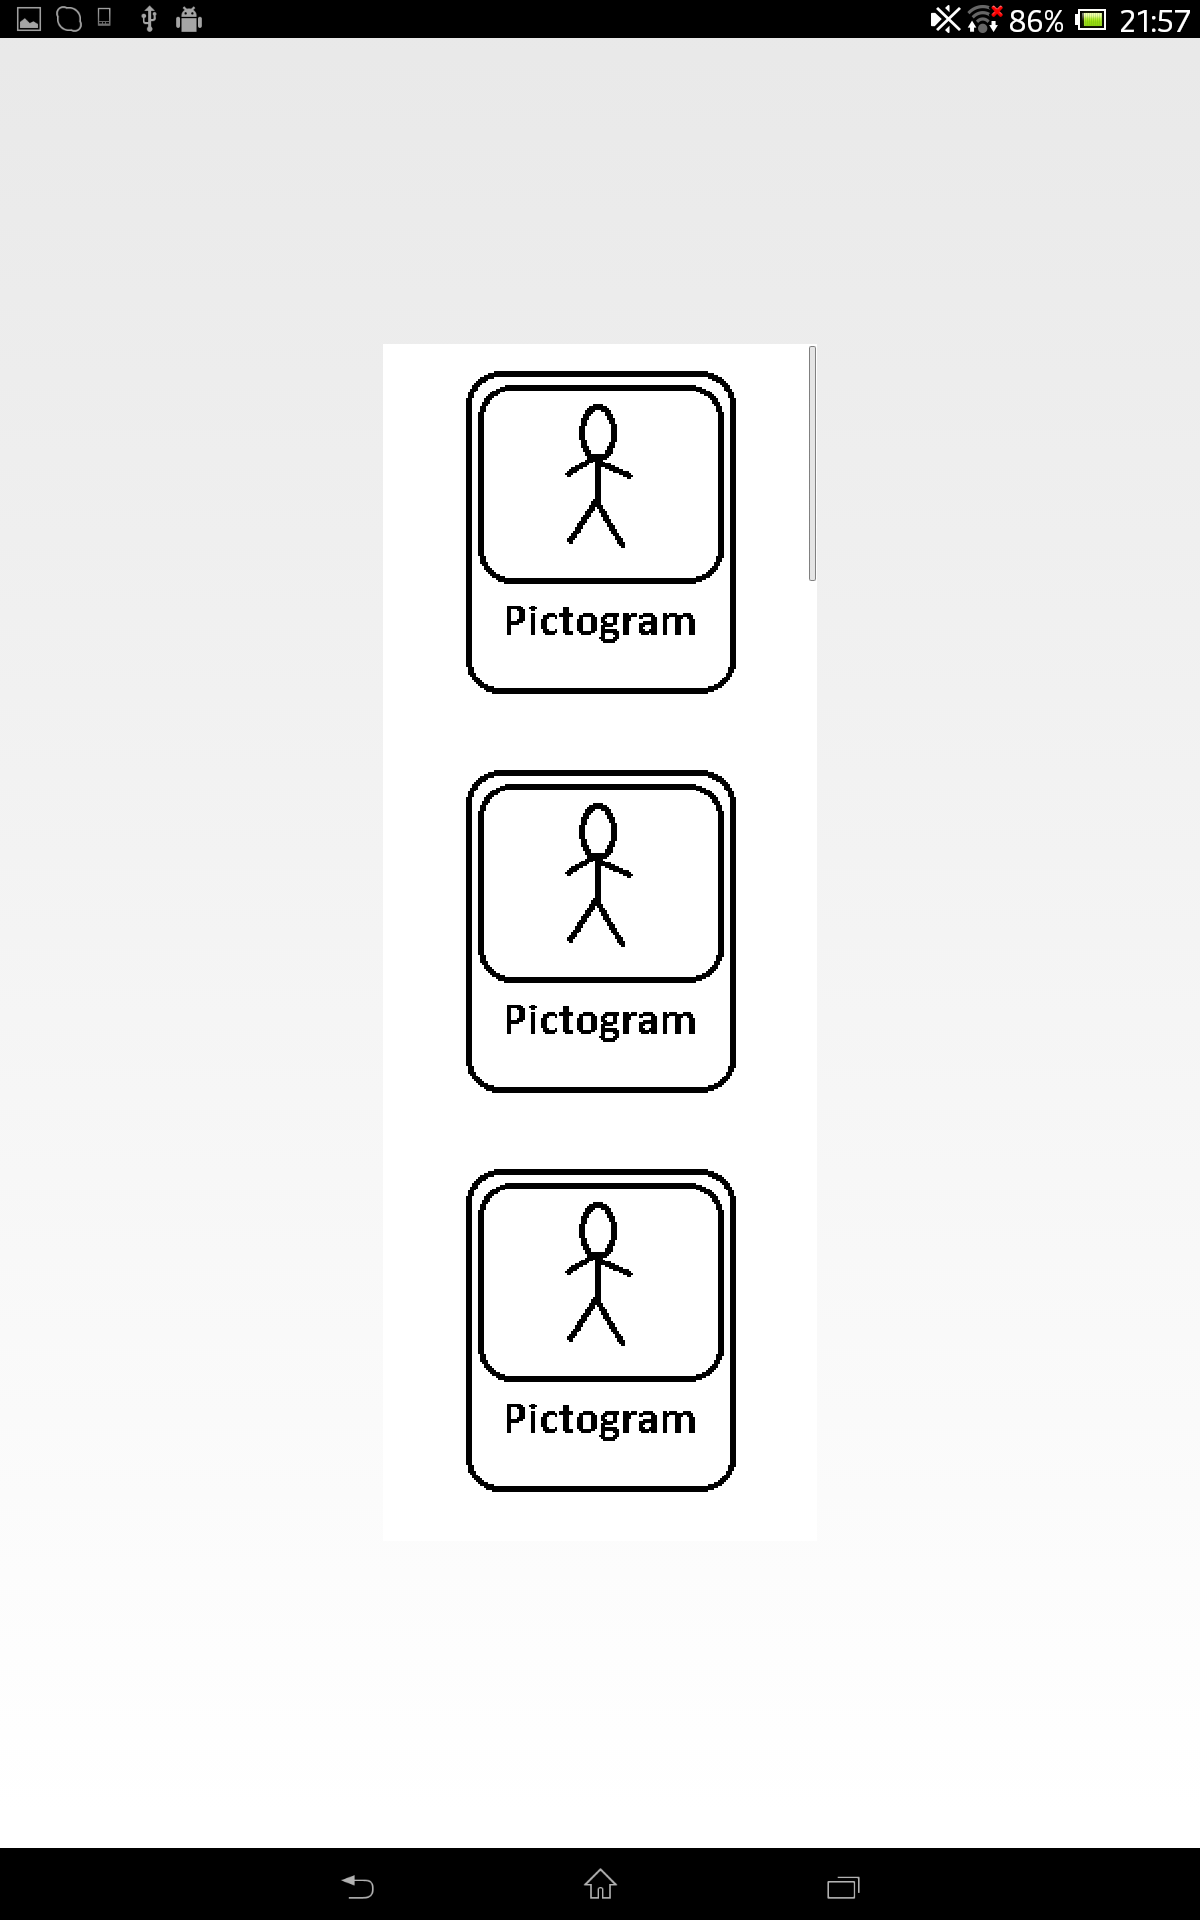
\includegraphics[scale=0.1]{Pics/Sprint3/portrait3pics.png}
\caption{A sequence displayed with 3 visible pictograms in portrait-mode}
\label{fig:portrait3pics}
\end{minipage}\hfill
\begin{minipage}{.45\textwidth}
\centering
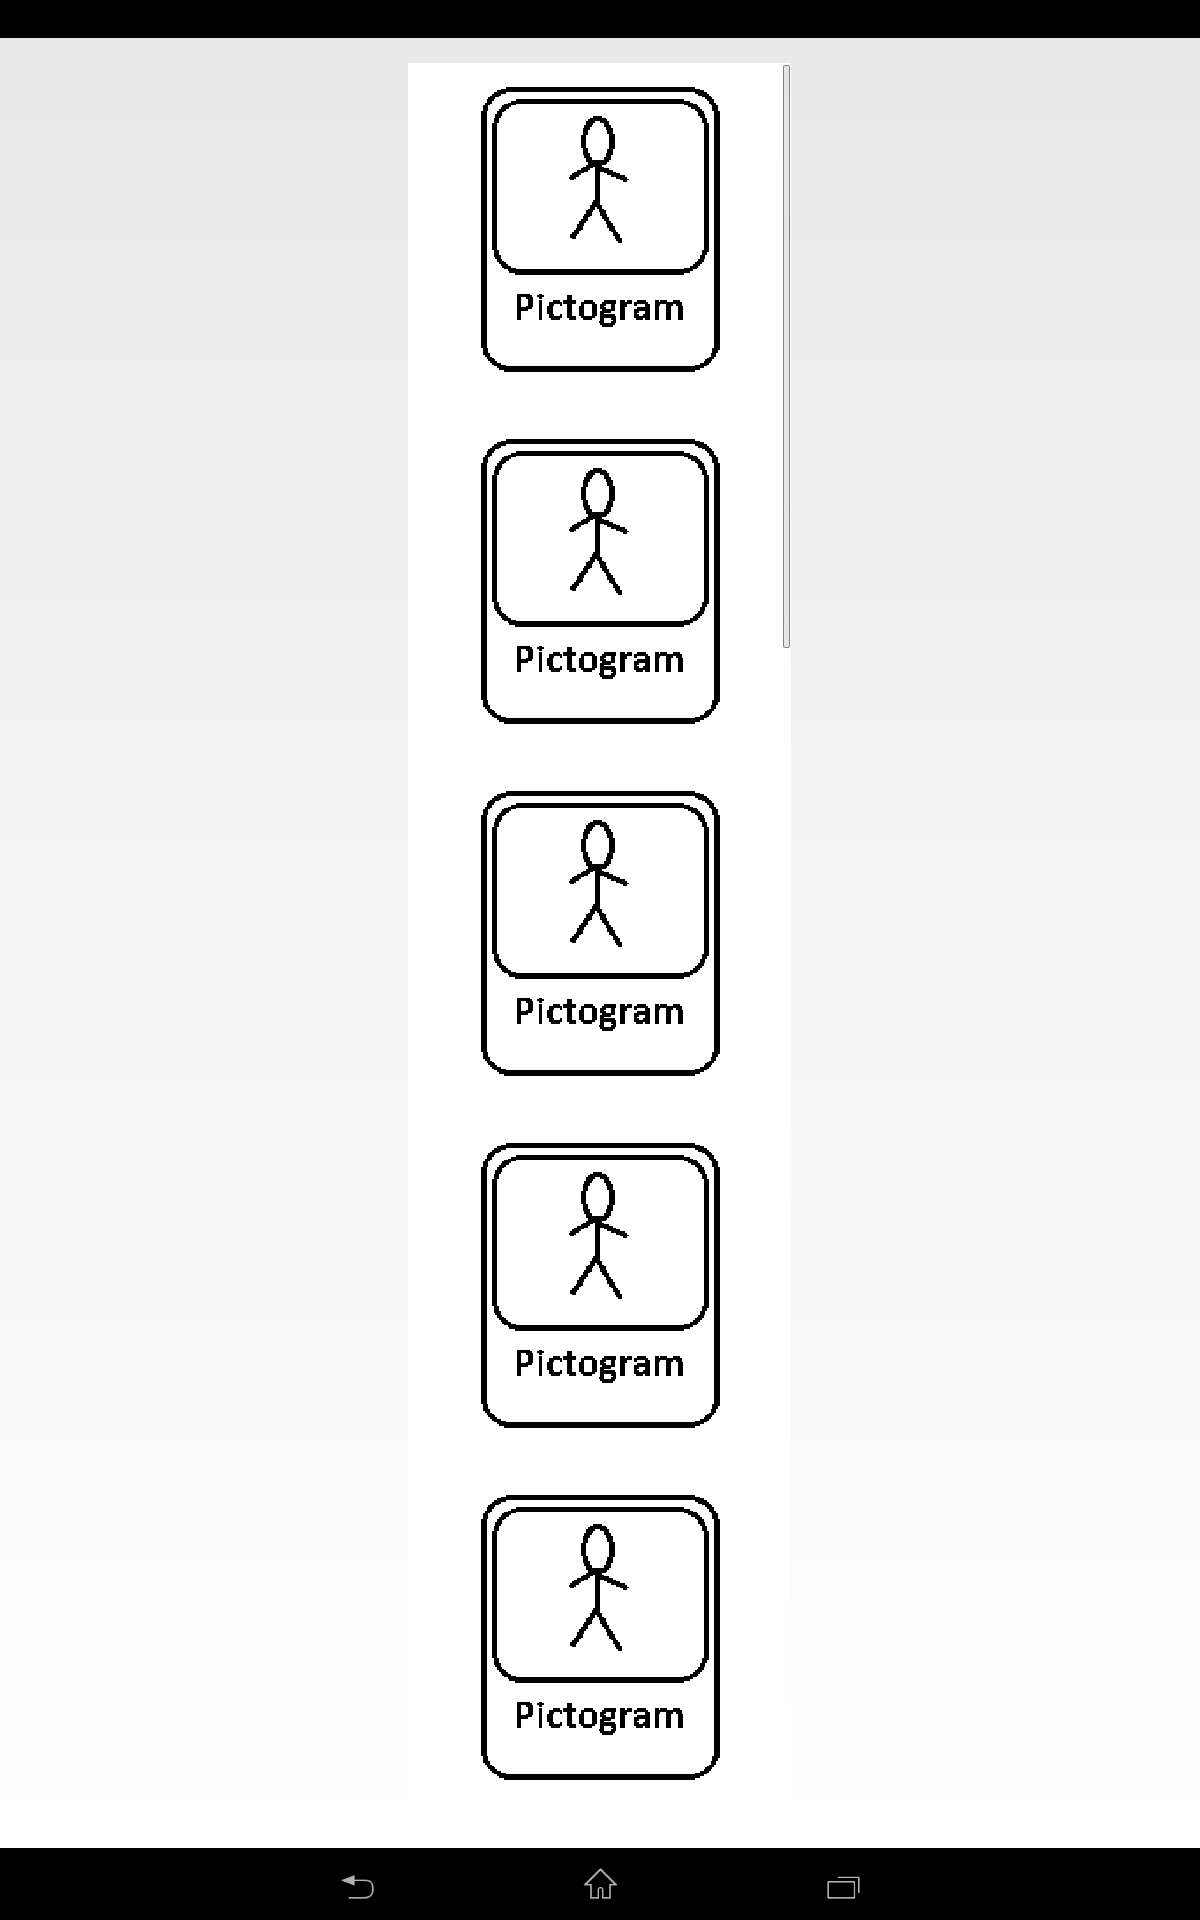
\includegraphics[scale=0.1]{Pics/Sprint3/portrait5pics.png}
\caption{A sequence displayed with 5 visible pictograms in portrait-mode}
\label{fig:portrait5pics}
\end{minipage}
\end{figure}















